\section{Effect of Mini-Batch Sampling on the Diagnostics}
\label{sec:sgd-noise-experiments}

The full-batch experiments isolate gradient interactions along a training
trajectory. With mini-batches, the same diagnostics also reflect which
examples enter each gradient estimate. Section~\ref{subsec:sampling-noise}
predicts that reducing batch size increases the magnitude of the negative
expected noise contribution and can weaken consecutive-gradient alignment. We test this
prediction first at fixed parameters, where sampling is the only source of
variation, and then during SGD, where the parameters also move. This separates
a change in gradient estimation from its consequences for accumulated
parameter displacement.

\subsection{Experimental Design}

We use the CIFAR-10 MLP and squared-error objective described in
Section~\ref{sec:gd-experiments}, with all $N=5{,}000$ training images.
For each of three independent initializations, a new full-batch GD run
at $\eta=0.02$ provides parameter states before training and after
1,000 and 2,000 updates. These update counts sample different portions of
the reference trajectories; they do not define common stability regimes
across initializations. At each saved state, we vary only the batch size,
$b\in\{32,128,512,2048,5000\}$.

The fixed-parameter comparison draws 32 independent sequences of 128
mini-batch gradients per condition, without updating the parameters.
The training comparison instead resumes SGD for 200 updates from each
saved state, with eight independent sampling repetitions per mini-batch
size and one full-batch GD continuation. Each batch is sampled uniformly
without replacement and redrawn independently at every step. The learning
rate remains 0.02, with no momentum, weight decay, clipping or schedule.
All batch sizes share the same starting parameters within each comparison.
The displacement origin is reset to that starting state, so $R_{200}$
measures accumulation over the 200-update continuation. Equal update counts
serve a diagnostic comparison, rather than a comparison of training efficiency.

Within each sampling repetition, batch sizes share prefixes of the same
random permutation; permutations are independent across steps and repetitions.
Parameters and gradients are FP32, diagnostic reductions are FP64, and TF32
is disabled. There is no augmentation or dropout. Figure summaries first
average repetitions within each initialization, then weight the three
initializations equally. Shading shows the range of these three means.
For the fixed-parameter cosine comparison, conditional 95\% intervals use
4,000 bootstrap resamples of whole sampling sequences, preserving dependence
between adjacent pairs. The SGD summaries describe the complete 200-update
window, without assuming stationary behavior within it.

\subsection{Batch Size and Alignment at Fixed Parameters}

At fixed parameters, consecutive gradients differ only because their
mini-batches differ. We compute the full gradient and per-example gradient
covariance over all 5,000 images, then evaluate
Eqs.~\eqref{eq:noise-expectation}--\eqref{eq:noise-cosine-approx}
without fitted constants. Across the 36 stochastic conditions, the measured
mean squared noise norm agrees with Eq.~\eqref{eq:finite-population-noise}
within 0.50\% relative error, and the mean noise contribution in
Eq.~\eqref{eq:noise-expectation} agrees within 0.74\%.

\begin{figure*}[!t]
  \centering
  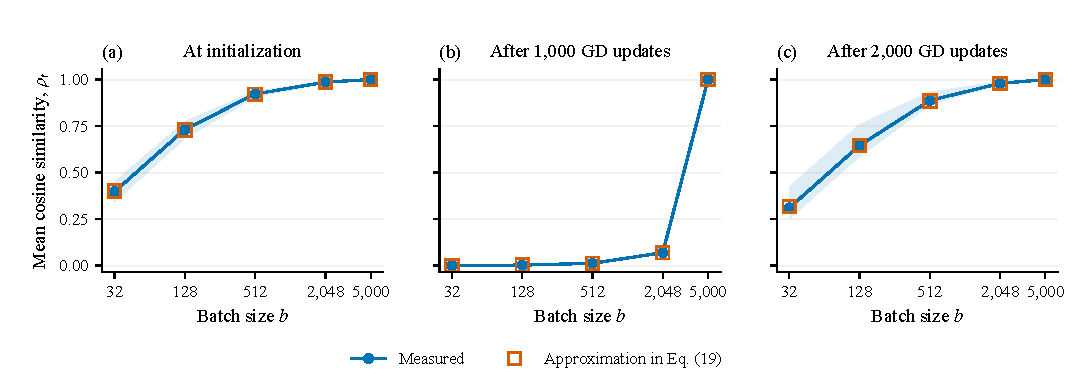
\includegraphics[width=\textwidth]{figures/analysis027/batch_size_fixed_parameters.pdf}
  \caption{Batch size and consecutive-gradient cosine at fixed parameters.
  Columns identify the saved GD state; no parameter updates occur during
  measurement. Circles show measurements and squares show
  Eq.~\eqref{eq:noise-cosine-approx}, evaluated per initialization before
  averaging. Shading is the range of three initialization means after averaging
  32 sampling sequences, not a confidence interval. The batch axis is logarithmic
  and lines guide the eye. At $b=5000$, every draw is the same full gradient.}
  \label{fig:sgd-frozen-calibration}
\end{figure*}

\begin{figure*}[!t]
  \centering
  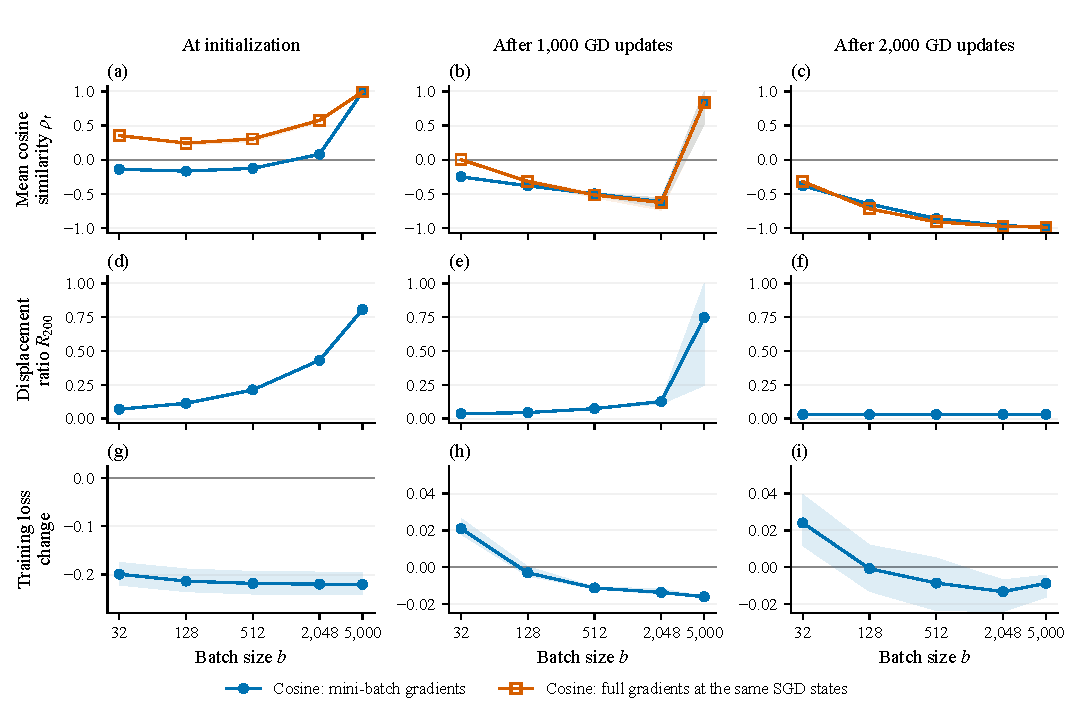
\includegraphics[width=\textwidth]{figures/analysis027/batch_size_sgd_outcomes.pdf}
  \caption{Outcomes over 200 SGD updates from each saved state. Top: mean
  consecutive cosine of mini-batch gradients (blue) and full gradients at the
  same SGD states (orange). Middle: normalized displacement $R_{200}$.
  Bottom: final minus initial training loss on all 5,000 images; positive
  values indicate an increase. Lines and shading show the mean and descriptive
  range of three initialization means after averaging sampling repetitions.
  Batch axes are logarithmic; $b=5000$ is full-batch GD. Loss axes use different ranges.}
  \label{fig:sgd-moving-geometry}
\end{figure*}

Figure~\ref{fig:sgd-frozen-calibration} shows the resulting effect on
$\rho_t$: smaller batches yield weaker alignment even though the parameters
never move. Equation~\eqref{eq:noise-cosine-approx} captures this dependence,
with maximum absolute error 0.0075. The agreement is approximate: its prediction
lies outside the conditional 95\% sampling interval in 21 of the 36 stochastic
conditions. The observed deviations therefore remain distinguishable from
sampling uncertainty.

The effect also depends on the training state. At batch size 2,048, the mean
cosine is 0.986 at initialization but only 0.069 at the state reached after
1,000 GD updates. Thus, even using over 40\% of this dataset in each batch
does not ensure strong alignment. Equation~\eqref{eq:noise-cosine-approx}
explains this dependence through the sampling variance relative to the
squared full-gradient norm. Batch size alone does not specify that balance.

\subsection{Alignment, Displacement and Loss during SGD}

Once training resumes, changing the batch size also changes the visited
parameters. Figure~\ref{fig:sgd-moving-geometry} summarizes consecutive-gradient
cosine, normalized displacement and training loss for all continuations.
To distinguish estimation noise from changes along the trajectory, we also
compute the full-data gradients at the same SGD parameter states and apply
the same cosine formula to them. These full gradients are used only for
measurement; each SGD update still uses its sampled mini-batch gradient.

From initialization, batch size 32 produces mean sampled cosine $-0.141$,
while the full gradients along the same trajectories have mean cosine
$+0.353$. Training loss nevertheless decreases. Negative sampled alignment
can therefore coexist with positive average full-gradient alignment and
objective progress. The full-batch continuation has mean cosine $0.994$,
showing that mini-batching changes both gradient estimation and the path
followed through the objective.

From the state after 2,000 GD updates, reducing the batch from 5,000 to 32
moves mean cosine from $-0.991$ to $-0.384$. Yet $R_{200}$ remains near
0.03 in both cases (0.0319 and 0.0303), so weaker consecutive reversal does
not translate into a larger fraction of retained displacement. Mean training
loss decreases by 0.0087 under full GD but increases by 0.0241 at batch 32;
the latter increase occurs in every initialization-specific mean. The batch
response is not uniformly monotonic: batch 2,048 attains a lower final loss
than full GD in all three initializations at this starting state.

These results connect the sampling argument in
Section~\ref{subsec:sampling-noise} to the displacement decomposition.
Noise can weaken alignment at fixed parameters, but during SGD the observed
cosine also reflects parameter motion. Its sign or proximity to zero does
not determine cumulative displacement or loss reduction. Accordingly,
$\eta\widehat\kappa_t$ retains the noise contribution identified in
Eq.~\eqref{eq:kappa-estimate}; interpreting it as curvature alone requires
that contribution to be small. These observations cover one MLP objective and learning rate over
200-update continuations; they do not define a general stability criterion.
